\begin{figure}[H]
    \centering


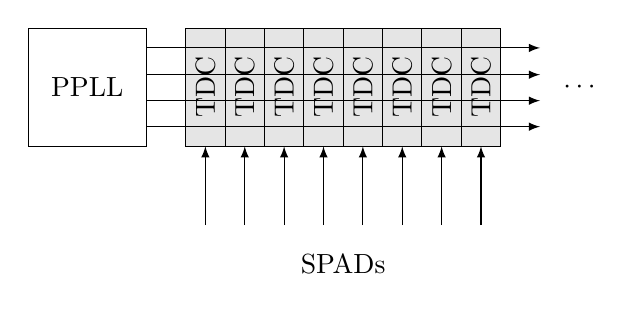
\begin{tikzpicture}

\draw  (-3.25,3) rectangle (-1.75,1.5) node[pos=.5]{PPLL};

\draw [fill=gray!20] (-1.25,3) rectangle (-0.75,1.5) node[pos=.5, rotate=90]{TDC};
\draw [fill=gray!20] (-0.75,3) rectangle (-0.25,1.5) node[pos=.5, rotate=90]{TDC};
\draw [fill=gray!20] (-0.25,3) rectangle (0.25,1.5) node[pos=.5, rotate=90]{TDC};
\draw [fill=gray!20] (0.25,3) rectangle (0.75,1.5) node[pos=.5, rotate=90]{TDC};
\draw [fill=gray!20] (0.75,3) rectangle (1.25,1.5) node[pos=.5, rotate=90]{TDC};
\draw [fill=gray!20] (1.25,3) rectangle (1.75,1.5) node[pos=.5, rotate=90]{TDC};
\draw [fill=gray!20] (1.75,3) rectangle (2.25,1.5) node[pos=.5, rotate=90]{TDC};
\draw [fill=gray!20] (2.25,3) rectangle (2.75,1.5) node[pos=.5, rotate=90]{TDC};

\draw [>=latex, ->] (-1.75,2.75) -- (3.25,2.75);
\draw [>=latex, ->] (-1.75,2.41) -- (3.25,2.41);
\draw [>=latex, ->] (-1.75,2.08) -- (3.25,2.08);
\draw [>=latex, ->] (-1.75,1.75) -- (3.25,1.75);

\draw [>=latex, ->] (-1,0.5) -- (-1,1.5);
\draw [>=latex, ->] (-0.5,0.5) -- (-0.5,1.5);
\draw [>=latex, ->] (0,0.5) -- (0,1.5);
\draw [>=latex, ->] (0.5,0.5) -- (0.5,1.5);
\draw [>=latex, ->] (1,0.5) -- (1,1.5);
\draw [>=latex, ->] (1.5,0.5) -- (1.5,1.5);
\draw [>=latex, ->] (2,0.5) -- (2,1.5);
\draw [>=latex, ->] (2.5,0.5) -- (2.5,1.5);

\node at (3.75,2.25) {$\cdots$};
\node at (0.75,0) {SPADs};
\end{tikzpicture}
    \caption{TDC line connected to PLL}
    \label{tkz:TDC_line_PLL}
\end{figure}